
% FIGURES
\begin{figure}[htb]
	\caption{\label{fig:1010} Forças internas atuando em um corpo em equilíbrio}
	\begin{center}
		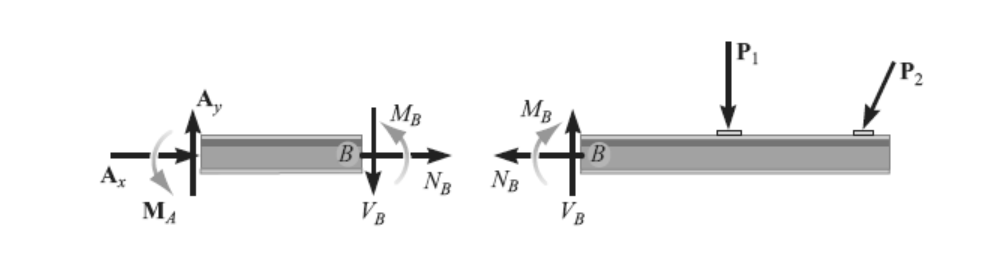
\includegraphics[width=\textwidth]{pictures/1010.png}
	\end{center}
	\fonte{\autocite{Hibbeler2010}}
\end{figure}


% EQUATIONS
\begin{equation}\label{eq:Eq_101}%
\mbox{\fontsize{17.28}{21.6}\selectfont\( %
\sum F_{x} = 0 \sum F_{y} = 0 \sum F_{z} = 0
\sum M_{x} = 0 \sum M_{y} = 0 \sum M_{z} = 0
\)} %
\end{equation}

\newline

sendo

$F_{x}$: Força de tração gerada pelos pneus

$\mu$: Coeficiente de atrito máximo do contato

W: Carga aplicada no eixo de tração


% DOUBLE EQUATIONS
\begin{equation}\label{eq:Eq_110}%
\mbox{\fontsize{17.28}{21.6}\selectfont\( %
\sum F_{x} = \sum F_{y} = \sum F_{z} = 0
\)} %
\end{equation}

\begin{equation}\label{eq:Eq_220}%
\mbox{\fontsize{17.28}{21.6}\selectfont\( %
\frac{V_{out}}{V_{in}} = \frac{k}{4}(\varepsilon_1 - \varepsilon_2 + \varepsilon_3 - \varepsilon_4)
\)} %
\end{equation}

\hfill

Onde:

$F_{i}$: Forças axiais aplicadas no corpo no eixo "i"

$M_{i}$: Momentos aplicados no corpo no eixo "i"


% TABLE GENERAL
\begin{table}[htb]
\caption[Funções utilizadas]{Funções utilizadas}
\label{tab-nivinv}
\resizebox{\textwidth}{!}{%
\begin{tabular}{p{2.6cm}p{6.0cm}p{2.25cm}p{3.40cm}}
  \toprule
   {Função} & \textbf{Descrição }  & \textbf{Parâmetros de entrada}  & \textbf{Parâmetros de saída}  \\
    \midrule
    numpy.array & Cria um objeto do numpy & Lista com valores & Vetor ndarray \\
    numpy.average & Obtem valor médio & Vetor ndarray & Valor médio \\
    numpy.std & Obtém desvio padrão & Vetor ndarray & Valor desvio padrão \\
    numpy.amax & Obtém valor máximo & Vetor ndarray & Valor máximo \\
    numpy.amin & Obtém valor mínimo & Vetor ndarray & Valor mínimo \\
   \bottomrule
\end{tabular}
}
\fonte{\textcite{van86} -- \showfont}
\end{table}


% TABLE FOR VALUES
\begin{table}[!ht]
    \caption[Exemplo de tabela utilizando o pacote \emph{siunitx} e \emph{resizebox}]{Exemplo
        de tabela utilizando o pacote \emph{siunitx} e \emph{resizebox}  -- \showfont.}
    \label{tab:SimulationResults}
    \centering
    \resizebox{\linewidth}{!}{%
        \begin{tabular}{cc|cc|cc} \toprule
            \multicolumn{2}{l}{\textbf{Fase A} } & \multicolumn{2}{l}{\textbf{Fase B}}
            & \multicolumn{2}{l}{\textbf{Fase C}} \\ \hline
            Parâmetro       & Valor       & Parâmetro        & Valor        & Parâmetro         & Valor            \\\hline
            $I_{La1}$&$\SI{2.9082866e+000}{\A}$&  $I_{Lb1}$&$\SI{3.3878432e+000}{\A}$& $I_{Lc1}$&$\SI{3.0354175e+000}{\A}$ \\
            $I_{La2}$&$\SI{2.9083278e+000}{\A}$&  $I_{Lb2}$&$\SI{3.3935604e+000}{\A}$& $I_{Lc2}$&$\SI{3.0238770e+000}{\A}$ \\
            $I_{La3}$&$\SI{2.9057255e+000}{\A}$&  $I_{Lb3}$&$\SI{3.3936165e+000}{\A}$& $I_{Lc3}$&$\SI{3.0252536e+000}{\A}$ \\
            $P_{a1}$& $\SI{625.50259e+00}{\W}$&  $P_{b1}$& $\SI{724.85424e+00}{\W}$& $P_{c1}$& $\SI{662.06883e+00}{\W}$ \\
            $P_{a2}$& $\SI{625.31121e+00}{\W}$&  $P_{b2}$& $\SI{725.62100e+00}{\W}$& $P_{c2}$& $\SI{660.36375e+00}{\W}$ \\
            $P_{a3}$& $\SI{625.96179e+00 }{\W}$&  $P_{b3}$& $\SI{725.28968e+00}{\W}$& $P_{c3}$& $\SI{660.14426e+00}{\W}$ \\
            $Q_{a1}$& $\SI{36.605745e+00 }{\VA}$&  $Q_{b1}$& $\SI{45.613691e+00}{\VA}$& $Q_{c1}$& $\SI{54.531747e+00}{\VA}$ \\
            $Q_{a2}$& $\SI{19.160357e+00}{\VA}$&  $Q_{b2}$& $\SI{36.608133e+00}{\VA}$& $Q_{c2}$& $\SI{19.939460e+00}{\VA}$ \\
            $Q_{a3}$& $\SI{18.867027e+00}{\VA}$&  $Q_{b3}$& $\SI{47.791169e+00}{\VA}$& $Q_{c3}$& $\SI{13.797842e+00}{\VA}$ \\
            $V_{Ca1}$&$\SI{400.04695e+00}{\V}$&  $V_{Cb1}$&$\SI{400.00862e+00}{\V}$& $V_{Cc1}$&$\SI{400.11656e+00}{\V}$ \\
            $V_{Ca2}$&$\SI{399.93041e+00}{\V}$&  $V_{Cb2}$&$\SI{400.05835e+00}{\V}$& $V_{Cc2}$&$\SI{399.97514e+00}{\V}$ \\
            $V_{Ca3}$&$\SI{400.02312e+00}{\V}$&  $V_{Cb3}$&$\SI{399.93403e+00}{\V}$& $V_{Cc3}$&$\SI{399.90881e+00}{\V}$ \\
            $I_{Ca1}$&$\SI{1.2605228e+000}{\A}$&  $I_{Cb1}$&$\SI{1.4684945e+000}{\A}$& $I_{Cc1}$&$\SI{1.3054048e+000}{\A}$ \\
            $I_{Ca2}$&$\SI{1.2661075e+000}{\A}$&  $I_{Cb2}$&$\SI{1.4720236e+000}{\A}$& $I_{Cc2}$&$\SI{1.3089556e+000}{\A}$ \\
            $I_{Ca3}$&$\SI{1.2598194e+000}{\A}$&  $I_{Cb3}$&$\SI{1.4708279e+000}{\A}$& $I_{Cc3}$&$\SI{1.3017673e+000}{\A}$ \\
            \bottomrule
        \end{tabular}}
\fonte{O autor -- \showfont}
\end{table}


% TABLE FOR VALUES
\begin{table}[!ht]
    \caption{Valores de massas utilizadas para aplicação das cargas nos dispositivos de flexão e torção}
    \label{tab:MassasUtilizadas}
    \centering
    \resizebox{\linewidth}{!}$ \\
            Fuso & $\SI{48.63}{\g}$ & $\SI{48.78}{\g}$ & $\SI{0.31}{\%}$ \\
            Peso 1 & $\SI{86.73}{\g}$ & $\SI{99.68}{\g}$ & $\SI{12.99}{\%}$ \\
            Peso 2 & $\SI{198.38}{\g}$ & $\SI{198.36}{\g}$ & $\SI{0.01}{\%}$ \\
            Peso 3 & $\SI{997.13}{\g}$ & $\SI{997.3}{\g}$ & $\SI{0.02}{\%}$ \\
            Peso 4 & $\SI{497.66}{\g}$ &$\SI{497.69}{\g}$ & $\SI{0.02}{\%}$ \\
            Peso 5 & $\SI{495.25}{\g}$ & $\SI{496.22}{\g}$ & $\SI{0.20}{\%}$ \\
            \bottomrule
        \end{tabular}}
\fonte{O autor 2022}
\end{table}